\documentclass[acmlarge, nonacm]{acmart}

\AtBeginDocument{
  \providecommand\BibTeX{{
    Bib\TeX}}}
    

\acmJournal{POMACS}
\acmVolume{37}
\acmNumber{4}
\acmArticle{1}
\acmMonth{8}
\usepackage{url}

\usepackage{listings}
\usepackage{xcolor}

\lstdefinestyle{kaleidoscope}{
  backgroundcolor=\color{white},
  basicstyle=\ttfamily\small,
  keywordstyle=\color{blue}\bfseries,
  commentstyle=\color{green!60!black},
  stringstyle=\color{orange},
  numbers=left,
  numberstyle=\tiny\color{gray},
  breaklines=true,
  frame=single,
  captionpos=b
}

\lstset{style=kaleidoscope}

\usepackage{etoolbox}
\newcommand{\studentinfo}{%
  \par\vspace{0.5em}
  \noindent\textbf{Student ID:} 2232602042 \\
  \textbf{Course:} CSE425 -- Concepts of Programming Languages \\
  \textbf{Section:} 1 \\
  \textbf{Semester:} Spring, 2026 \\
  \textbf{Instructor:} Dr. Md. Shahriar Karim [MSK1]
}




\begin{document}
\title{A Technical Report on the Implementation of Kaleidoscope Programming Language with LLVM}

\author{Md. Nafis Muktashid Arpon}
\email{nafis.arpon@northsouth.edu}
\affiliation{%
  \department{Department of Electrical and Computer Engineering}
  \institution{North South University}
  \city{Dhaka}
  \country{Bangladesh}
}


\maketitle
\studentinfo\\

\section*{Abstract}
	This technical report outlines the implementation of the Kaleidoscope programming language frontend with LLVM. It includes lexer, perser, and additional key language features stated in the LLVM tutorial \citep{llvm}. This report also illustrates how the language can be extended with minimal changes with two cases, boolean literals and a modulo operator.

\section{Introduction}
The LLVM Tutorial \cite{llvm} introduces the simple "Kaleidoscope" language showing the range of language design and LLVM-specific ideas, and explaining the code for it. The object is to establish an understanding between the theoretical concepts from the course and a working implementation of a compiler based programming language. The complete source code for this implementation, including all extensions and modifications, is publicly available on GitHub \cite{github}.

\section{Theoretical Framework}
\subsection{Lexical Analysis}
A lexical analyzer is essentially a pattern matcher. A pattern matcher attempts to find a substring of a given string of characters that matches a given character pattern. It is done by a lexer. A compiler takes a raw source code and serves as the front end of a syntax analyzer. This is achieved by scanning the raw source code and convert it into a sequence of lexemes and tokens. A lexeme is an actual substring of characters and token is the stratified lexemes. For instance, integers form the token type \verb|INT_LITERAL| and variable names form a token type \verb|IDENTIFIER|. Different programming language contains different token types. C has 6 different token types.

\begin{itemize}
\item{\textbf{KEYWORD:}} These are the words that have special meaning in the language implementation and reserved for that purpose only. Such as, \verb|main, if, else, for, break.|
\item{\textbf{IDENTIFIER:}} These are usually the alphanumeric characters and character strings that identifies the user defined elements of the program, such as functions and variables. Programming languages impose rules to define these identifiers. For example, in C, the first character of an identifier must be alphabet or underscore without any whitespace present.
\item{\textbf{OPERATORS:}} These are symbols that act as interface and determines the type of operation to be carried out. Example includes, +, -, *, /, ==, <=, >=, !=
\item{\textbf{CONSTANT:}} These remains fixed meaning do not change during the execution of the program. The primary types of constants in C are integer constants, floating-point constants, and string constants.
\item{\textbf{STRING:}} They are sequences of characters enclosed by double quotes.
\item{\textbf{PUNCTUATION:}} These work in separating different sections from one another. Brackets, terminators, and separators are examples f punctuation.
\end{itemize}

For theoretical implementation, a valid set of lexemes, or a vocabulary, is specified. We use regular expressions and finite automata to design the lexer. There are various tools avalibale that directly generate the lexer and parser, such as Lex and Flex. The foundation for lexer includes,
\begin{itemize}
\item{\textbf{REGULAR EXPRESSION:}} This describes the patterns of valid tokens. i.e. \verb|IDENTIFIER, OPERATOR|
\item{\textbf{REGULAR GRAMMARS:}} This provides us a formal basis for expressing how tokens are formed.
\item{\textbf{FINITE AUTOMATA:}} This act as the computation model that recognizes the regular languages. A lexer can be viewed as a \textit{Deterministic Finite Automata} (DFA) that transitions between states based on the character input and accepts when a valid token is found.
\end{itemize}

A lexer for any programming language can be derive by first expressing token patterns using regular expressions then converting these expression to an \textit{Non-deterministic Finite Automata} (NFA), and finally transforming it to a DFA for efficient implementation. Even though the Kaleidoscope language lexer is hand-written, the same theoretical principle stands.

\subsection{Syntax Analysis}
The part of the process of analyzing syntax that is referred to as syntax analysis is often called parsing. Persers for programming languages construct parse trees for given programs \cite{sebesta}. A syntax analyzer works with the tokens generated by the lexical analyzer. The parser checks if the sequence of token forms a valid syntactical representation or not. Initially, the syntax of a programming language was described with \textit{Context-Free Grammar} (CFG). Later, a new modified notation called \textit{Backus-Naur Form} (BNF) was introduced. Using BNF description as opposed to using some informal syntax description, has at least three compelling advantages. First, BNF descriptions of the syntax of programs are clear and concise, for both humans and for software systems that use them. Second, the BNF description can be used as the direct basis for the syntax analyzer. Third, implementations based on BNF are relatively easy to maintain because of their modularity \cite{sebesta}.

A metalanguage is a language that is used to describe another language. BNF is a metalanguage for programming languages. Its description is a collection of rules using symbols. BNF has 2 types of symbols--terminal and non-terminal. Terminal symbols are tokens and lexemes of any rule. Non-terminal symbols are abstractions in BNF description.

A parse tree is build to show how the input is derived from the start symbol of the grammar. A more compact version of the parse tree is the \textit{Abstract Syntax Tree} (AST), where all the non-terminals are eliminated. The AST serves as the main input of the later phases such as semantic analysis and code generation.

\subsection{Intermediate Representation}
Most modern compilers use one or more \textit{Intermediate Representations} (IR) between the high-level source code and the final machine code. IR is and low-level, language-independent representation of the source code that is easier to analyze and transform.

A ubiquitous IR style is introduced in our course is \textit{Three Address Code} (AST). In AST, the instructions use at most one operator and up to three operands. This way complex expression can be broken down in into simple steps using temporary variables. An example \verb|x = a + b + c| can be followed.

\begin{lstlisting}
t1 = a + b
t2 = t1 + c
x = t2
\end{lstlisting}

LLVM IR works in a similar function but more structured way. It uses \textit{Static Single Assignment} (SSA) form. The name somewhat indicates how it operates. It works by assigning each logical variable exactly once. Thus if a new value is appeared, a new SSA is created. One important SSA operation is the $\phi$ Function. The execution of $\phi$ function requires \textit{remembering} from which block the control came. The $\phi$ function takes on the value corresponding to the input control block. The benefit of explicit dataflow relationship of SSA makes very suitable for a front-end like Kaleidoscope.

\subsection{IR Optimizations}
Once the AST in generated by the Syntax analyzer, optimizations can be resolved to improve the performance of the code without compromising any unwanted behaviour of the program. Worldwide many optimization techniques are widely recognized. Some of them are follows:

\begin{itemize}
\item{\textbf{Constant Folding:}} The compiler resolves expressions involving constants at compile time instead of runtime.
\begin{lstlisting}
x = 3 + 4 + 5;
\end{lstlisting}
Compiler will fold the value of \verb|x| in compile time and hold the value 12 directly in the IR.

\item{\textbf{Constant Propagation:}} The compiler resolves the use of any known variable that holding a constant value by substituting its constant to other places.
\begin{lstlisting}
x = 3;
y = x + 9;
\end{lstlisting}
Compiler will substitute \verb|x| and by the use of other optimization techniques \verb|y| will have the value of 12 and \verb|x| will be eliminated from the runtime execution.

\item{\textbf{Copy Folding:}} The compiler resolves any duplicate variable by using the original instance.
\begin{lstlisting}
x = a;
y = a + 9;
\end{lstlisting}
Compiler will simplify the equation by writing \verb|y = x + 9;| 

\item{\textbf{Dead Code Elimination:}} The compiler resolves any unused, non-harmful part of code by removing it.
\begin{lstlisting}[language=C++]
x = func();
y = 3 + 9;
return y;
\end{lstlisting}
Since \verb|x| is never used, compiler will remove the code to improve the runtime of the program.
\end{itemize}



\section{The LLVM Project}
The LLVM Project is a collection of modular and reusable compiler and toolchain technologies. LLVM stands for Low Level Virtual Machine. The name "LLVM" itself is not an acronym but full name of the project.It is a SSA-based compilation strategy capable of supporting both static and dynamic compilation of arbitrary programming language. It is a compiler infrastructure that separates the front-end and back-end of the compiler design process. If the front-end of a language is implemented, then the rest from IR to machine code generation is handled by LLVM itself. \cite{llvm}



\section{Kaleidoscope Language}
The Kaleidoscope language is a procedural toy language that supports numeric expressions, variables, function definitions. Kaleidoscope uses a 64-bit floating point with all values are implicitly double precision without type declarations.



\section{Implementation}
\subsection{Lexer Design}
The lexer is defined by five different token type: \verb|tok_eof, tok_def, tok_extern, tok_identifier, tok_number|. Symbols that are not defined as any token are returned by their ASCII codes. Global statis variables \verb|string IdentifierStr| and \verb|double NumVal| are also declared to hold the value for current token for identifier and number, respectively.

\begin{lstlisting}[language=C++]
// The lexer returns tokens [0-255] if it is an unknown character, otherwise one
// of these for known things.
enum Token {
  tok_eof = -1,

  // commands
  tok_def = -2,
  tok_extern = -3,

  // primary
  tok_identifier = -4,
  tok_number = -5,
};

static std::string IdentifierStr; // Filled in if tok_identifier
static double NumVal;             // Filled in if tok_number
\end{lstlisting}

The lexer reads one character at a time, skipping whitespace, grouping alphabetic sequences into identifiers and numeric sequences into number literals. This characteristics replicates a DFA. It enters an "identifier state" for alphabetic input and a "number state" for digits. The lexical analyzer is defined in a single function called \verb|gettok()|. It returns the next token from the standard input. The function maintains a static variable name \verb|LastChar| which holds the last character read from input. A lookahead is used to determine token boundaries using the \verb|gettok()| funciton. For identifiers, the lexer consumes through alphanumeric characters untill a non-identifier character comes. For numbers, the lexer continues through digits and decimal point.

\begin{itemize}
\item{\textbf{Identifiers:}} If \verb|LastChar| is alphabet, the lexer reads the whole alphanumeric sequence and stores it in \verb|IdentifierStr| and compares it against reserved words. Upon matching it returns the token else \verb|tok_identifer| and the name store in \verb|IdentifierStr| is returned. 
\begin{lstlisting}[language=C++]
if (isalpha(LastChar)) { // identifier: [a-zA-Z][a-zA-Z0-9]*
  IdentifierStr = LastChar;
  while (isalnum((LastChar = getchar())))
    IdentifierStr += LastChar;

  if (IdentifierStr == "def")
    return tok_def;
  if (IdentifierStr == "extern")
    return tok_extern;
  return tok_identifier;
}

\end{lstlisting}

\item{\textbf{Numbers:}} If \verb|LastChar| is digit or dot, the lexer reads the sequence of digits and dots and stores it in the temporary variable \verb|NumStr|. Then it is converted into a floating-point value and saved in the \verb|NumVal|. Then the lexer returns the token \verb|tok_number|.
\begin{lstlisting}[language=C++]
if (isdigit(LastChar) || LastChar == '.') {   // Number: [0-9.]+
  std::string NumStr;
  do {
    NumStr += LastChar;
    LastChar = getchar();
  } while (isdigit(LastChar) || LastChar == '.');

  NumVal = strtod(NumStr.c_str(), 0);
  return tok_number;
}
\end{lstlisting}

\item{\textbf{Comments:}} If '$\#$', then the rest of the line is treated as a comment. \verb|getchar()| is repeatedly called until newline, return or end-of-file.
\begin{lstlisting}[language=C++]
if (LastChar == '#') {
  // Comment until end of line.
  do
    LastChar = getchar();
  while (LastChar != EOF && LastChar != '\n' && LastChar != '\r');

  if (LastChar != EOF)
    return gettok();
}
\end{lstlisting}

\item{\textbf{End Of File:}} If \verb|LastChar| is EOF then token \verb|tok_eof| is returned.
\begin{lstlisting}[language=C++]
  // Check for end of file.  Don't eat the EOF.
  if (LastChar == EOF)
    return tok_eof;

  // Otherwise, just return the character as its ascii value.
  int ThisChar = LastChar;
  LastChar = getchar();
  return ThisChar;
}
\end{lstlisting}
\end{itemize}


\subsection{Parser Design}
The output tokens from the lexer is used as input for  the parser. The parser then creates an AST. The parser reads tokens, verifies them and generates the AST representing the hierarchical structure. The grammar of Kaleidoscope defined for lexer the Parser as follows.
\begin{lstlisting}
<program>           ::= (<definition> | <extern> | <toplevelexpr>)*
<numberexpr>        ::= <number>
<parenexpr>         ::= '(' <expression> ')'
<identifierexpr>    ::= <identifier> | <identifier> '(' <expression>* ')'
<primary>           ::= <identifierexpr> | <numberexpr> | <parenexpr>
<binoprhs>          ::= ('+' <primary>)*
<expression>        ::= <primary> <binoprhs>
<prototype>         ::= <id> '(' <id>* ')'
<definition>        ::= 'def' <prototype> <expression>
<toplevelexpr>      ::= <expression>
<external>          ::= 'extern' <prototype>
<top>               ::= <definition> | <external> | <expression> | ';'
\end{lstlisting}

To create the AST, parser uses a combination of two different type of parsing. \textit{Recursive Descent Parsing} and \textit{Operator Precedence Parsing}. The AST captures structures and behaviours in a way that later stages for compiler is easy to interpret. Kaleidoscope has three primary language constructs. Expressions, Prototypes, and Functions. And \verb|ExporAST| is the common base class which all the expression nodes are inherited.
\begin{itemize}
\item{\textbf{NumberExprAST:}} This refers to the numeric literals and stores the value.
\item{\textbf{VariableExprAST:}} This refers to the variables and stores the variable name.
\item{\textbf{BinaryExprAST:}} This refers to the binary operations and stores the operator characters and points to the LHS and RHS sub-expressions.
\item{\textbf{CallExprAST:}} This refers to the function calls and stores the callee name with vector of arguments.
\item{\textbf{PrototypeAST:}} This refers to the function prototype and stores the function name and the list of arguments.
\item{\textbf{FunctionAST:}} This refers to the full function definition combined with \verb|PrototypeAST| and \verb|ExprAST|.
\end{itemize}

\begin{lstlisting}[language=C++]
/// ExprAST - Base class for all expression nodes.
class ExprAST {
public:
  virtual ~ExprAST() = default;
};

/// NumberExprAST - Expression class for numeric literals like "1.0".
class NumberExprAST : public ExprAST {
  double Val;

public:
  NumberExprAST(double Val) : Val(Val) {}
};

/// VariableExprAST - Expression class for referencing a variable, like "a".
class VariableExprAST : public ExprAST {
  std::string Name;

public:
  VariableExprAST(const std::string &Name) : Name(Name) {}
};

/// BinaryExprAST - Expression class for a binary operator.
class BinaryExprAST : public ExprAST {
  char Op;
  std::unique_ptr<ExprAST> LHS, RHS;

public:
  BinaryExprAST(char Op, std::unique_ptr<ExprAST> LHS,
                std::unique_ptr<ExprAST> RHS)
    : Op(Op), LHS(std::move(LHS)), RHS(std::move(RHS)) {}
};

/// CallExprAST - Expression class for function calls.
class CallExprAST : public ExprAST {
  std::string Callee;
  std::vector<std::unique_ptr<ExprAST>> Args;

public:
  CallExprAST(const std::string &Callee,
              std::vector<std::unique_ptr<ExprAST>> Args)
    : Callee(Callee), Args(std::move(Args)) {}
};

/// PrototypeAST - This class represents the "prototype" for a function,
/// which captures its name, and its argument names (thus implicitly the number
/// of arguments the function takes).
class PrototypeAST {
  std::string Name;
  std::vector<std::string> Args;

public:
  PrototypeAST(const std::string &Name, std::vector<std::string> Args)
    : Name(Name), Args(std::move(Args)) {}

  const std::string &getName() const { return Name; }
};

/// FunctionAST - This class represents a function definition itself.
class FunctionAST {
  std::unique_ptr<PrototypeAST> Proto;
  std::unique_ptr<ExprAST> Body;

public:
  FunctionAST(std::unique_ptr<PrototypeAST> Proto,
              std::unique_ptr<ExprAST> Body)
    : Proto(std::move(Proto)), Body(std::move(Body)) {}
};
\end{lstlisting}

\textbf{Parsing Function:} All the grammar rules in the parser are a function individually and they must be defined.
\begin{itemize}
\item{\textbf{ParseNumberExpr():}} This function handles the numeric literals. This creates a NumberExprAST object and returns it.
\begin{lstlisting}[language=C++]
/// numberexpr ::= number
static std::unique_ptr<ExprAST> ParseNumberExpr() {
  auto Result = std::make_unique<NumberExprAST>(NumVal);
  getNextToken(); // consume the number
  return std::move(Result);
}
\end{lstlisting}

\item{\textbf{ParseParenExpr():}} This function handles expressions with parenthesis and parses the sub-expression. Then it returns the sub-expression.
\begin{lstlisting}[language=C++]
/// parenexpr ::= '(' expression ')'
static std::unique_ptr<ExprAST> ParseParenExpr() {
  getNextToken(); // eat (.
  auto V = ParseExpression();
  if (!V)
    return nullptr;

  if (CurTok != ')')
    return LogError("expected ')'");
  getNextToken(); // eat ).
  return V;
}
\end{lstlisting}

\item{\textbf{ParseIdentifierExpr():}} This function handles both function calls and variable references and returns a \verb|CallExprAST| object.
\begin{lstlisting}[language=C++]
/// identifierexpr
///   ::= identifier
///   ::= identifier '(' expression* ')'
static std::unique_ptr<ExprAST> ParseIdentifierExpr() {
  std::string IdName = IdentifierStr;

  getNextToken();  // eat identifier.

  if (CurTok != '(') // Simple variable ref.
    return std::make_unique<VariableExprAST>(IdName);

  // Call.
  getNextToken();  // eat (
  std::vector<std::unique_ptr<ExprAST>> Args;
  if (CurTok != ')') {
    while (true) {
      if (auto Arg = ParseExpression())
        Args.push_back(std::move(Arg));
      else
        return nullptr;

      if (CurTok == ')')
        break;

      if (CurTok != ',')
        return LogError("Expected ')' or ',' in argument list");
      getNextToken();
    }
  }

  // Eat the ')'.
  getNextToken();

  return std::make_unique<CallExprAST>(IdName, std::move(Args));
}
\end{lstlisting}

\item{\textbf{ParsePrimary():}} This function uses a switch statement to work as an entry point for all these functions.
\begin{lstlisting}[language=C++]
/// primary
///   ::= identifierexpr
///   ::= numberexpr
///   ::= parenexpr
static std::unique_ptr<ExprAST> ParsePrimary() {
  switch (CurTok) {
  default:
    return LogError("unknown token when expecting an expression");
  case tok_identifier:
    return ParseIdentifierExpr();
  case tok_number:
    return ParseNumberExpr();
  case '(':
    return ParseParenExpr();
  }
}
\end{lstlisting}
\end{itemize} 

\textbf{Operator Precedence for Binary Expressions:} Binary expressions are often times ambiguous and require special handling because of operator precedence and associativity. Kaleidoscope uses a precedence table named \verb|BinopPrecedence| that stores the precedence of the operators. The \verb|GetTokPrecedence()| function returns the precedence of the current token if it is a binary operator, else it returns -1.
\begin{itemize}
\item{\textbf{ParseExpression():}} This function is the core that is used to parse binary expression with operator precedence. The function returns ParseBinOpRHS() function with 0 and LHS as arguments.

\item{\textbf{ParseBinOpRHS():}} This function parses the rest of the expression containing [BinOp, PrimaryExpr] pairs according to the precedence rules.
\end{itemize}

\textbf{Parsing Top Level input and Prototypes:}
\begin{itemize}
\item{\textbf{ParsePrototype():}} This function parses function prototypes.
\item{\textbf{ParseDefinition():}} This function handles function definition. This uses \verb|ParsePrototypeAST()| function and returns FunctionAST.
\item{\textbf{ParseExtern():}} This function is used for the extern declarations.
\item{\textbf{ParseTopLevelExpr():}} This function parses the top level expressions and transforms them into \verb|FucntionAST|.
\end{itemize}

\begin{figure}[H]
  \centering
  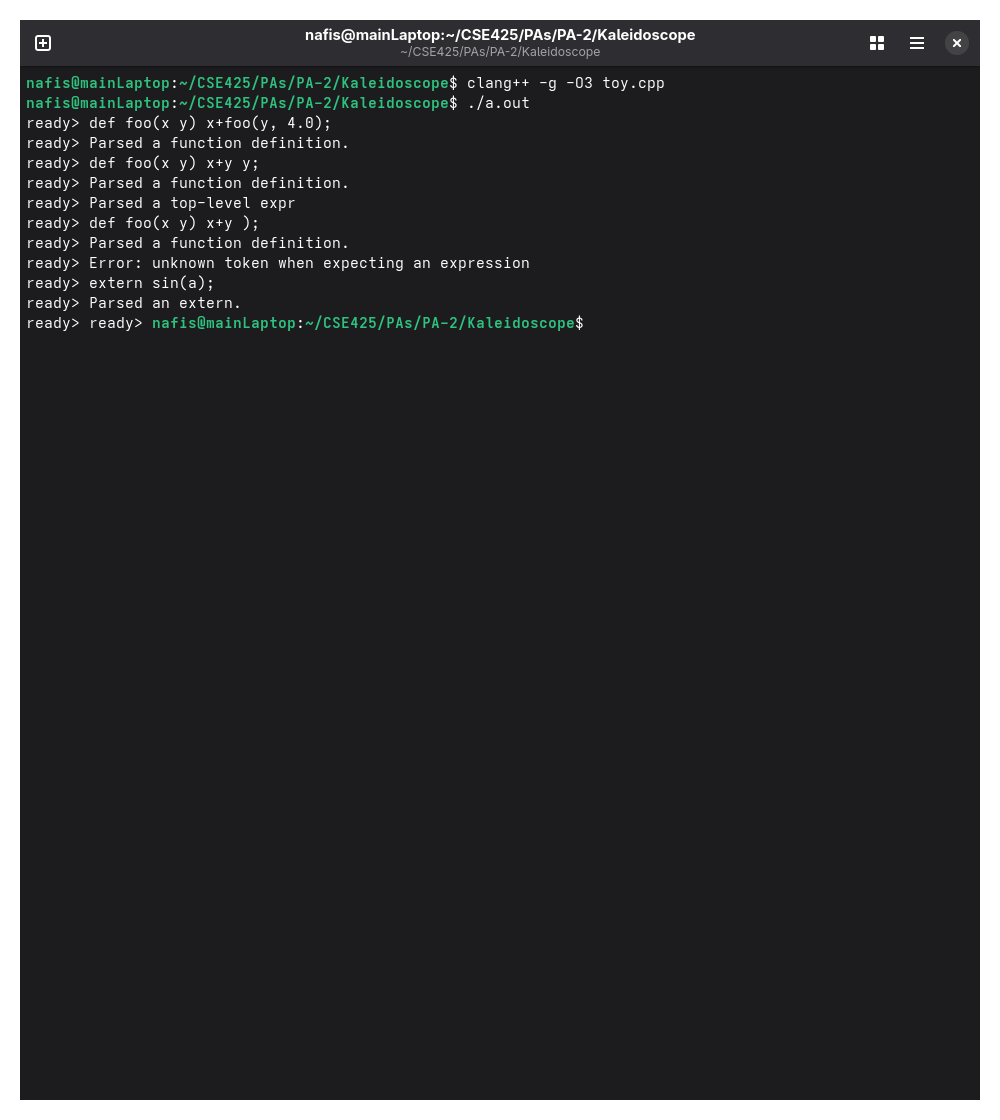
\includegraphics[width=0.55\linewidth]{./ch-2-1.png}
  \caption{Kaleidoscope Terminal Output for Parse}
  \label{fig:ch1-output}
\end{figure}


\subsection{Code Generation using LLVM IR}
The generated AST from the parse is taken as input for IR. Code generation converts the AST into LLVM IR. This LLVM IR is a low-level instruction set that can be optimized and executed on multiple target architectures. Each AST node implements a \verb|codegen()| method that produces an \verb|llvm:Value*| representing the IR value. LLVM utilities such as \verb|TheModule, Builder| and \verb|NamedValues| are used to manage IR construction.

\textbf{Expression Code Generation:} Each expression AST implements its own \verb|codegen()| method.
\begin{itemize}
\item{\textbf{Number:}} Numeric constants are represented with the ConstantFP class, which holds the numeric value in an APFloat internally.
\begin{lstlisting}[language=C++]
Value *NumberExprAST::codegen() {
  return ConstantFP::get(*TheContext, APFloat(Val));
}
\end{lstlisting}

\item{\textbf{Variables:}} Variables are looked up by their names in \verb|NamedValues|. If not found throws an "Unknown variable name" error.
\begin{lstlisting}[language=C++]
Value *VariableExprAST::codegen() {
  // Look this variable up in the function.
  Value *V = NamedValues[Name];
  if (!V)
    LogErrorV("Unknown variable name");
  return V;
}
\end{lstlisting}

\item{\textbf{Binary Operators:}} We recursively give code for the left-hand side and right-hand side. Then, it uses IRBuilder to create the instruction according to the operator.
\begin{lstlisting}[language=C++]
Value *BinaryExprAST::codegen() {
  Value *L = LHS->codegen();
  Value *R = RHS->codegen();
  if (!L || !R)
    return nullptr;

  switch (Op) {
  case '+':
    return Builder->CreateFAdd(L, R, "addtmp");
  case '-':
    return Builder->CreateFSub(L, R, "subtmp");
  case '*':
    return Builder->CreateFMul(L, R, "multmp");
  case '<':
    L = Builder->CreateFCmpULT(L, R, "cmptmp");
    // Convert bool 0/1 to double 0.0 or 1.0
    return Builder->CreateUIToFP(L, Type::getDoubleTy(*TheContext),
                                 "booltmp");
  default:
    return LogErrorV("invalid binary operator");
  }
}
\end{lstlisting}

\item{\textbf{Function Calls:}} This function looks up the callee and check if the number of arguments matches, recursively generate code for each argument and then emit a call instruction.
\begin{lstlisting}[language=C++]
Value *CallExprAST::codegen() {
  // Look up the name in the global module table.
  Function *CalleeF = TheModule->getFunction(Callee);
  if (!CalleeF)
    return LogErrorV("Unknown function referenced");

  // If argument mismatch error.
  if (CalleeF->arg_size() != Args.size())
    return LogErrorV("Incorrect # arguments passed");

  std::vector<Value *> ArgsV;
  for (unsigned i = 0, e = Args.size(); i != e; ++i) {
    ArgsV.push_back(Args[i]->codegen());
    if (!ArgsV.back())
      return nullptr;
  }

  return Builder->CreateCall(CalleeF, ArgsV, "calltmp");
}
\end{lstlisting}
\end{itemize}

\begin{figure}[H]
  \centering
  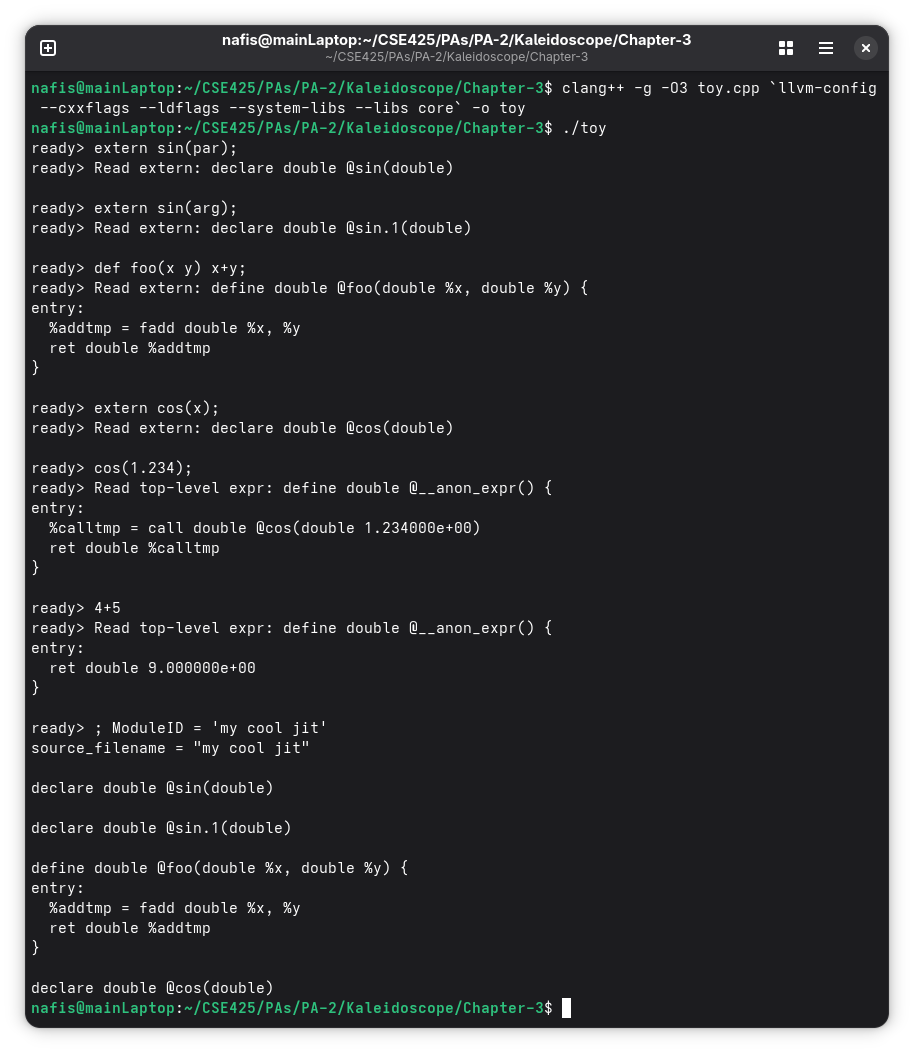
\includegraphics[width=0.55\linewidth]{./Ch-3.png}
  \caption{Kaleidoscope Terminal Output for IR Code Generation}
  \label{fig:ch1-output}
\end{figure}

\textbf{Function Code Generation:} 
\begin{itemize}
\item{\textbf{Prototypes:}} This describe the function’s name and argument list. Their \verb|codegen()| constructs a \verb|FunctionType| of the form \verb|double(double, ...)|. Then it creates an LLVM Function with external linkage and inserts it into \verb|TheModule|. The name of each of the function’s arguments is set according to the names given in the Prototype.
\item{\textbf{Function definitions:}} First look up an existing IR function with the same name, if none exists, it call the prototype’s \verb|codegen()| to create it. If there is no error, the LLVM ret instruction completes the function. Lastly function is built, LLVM provided \verb|verifyFunction()| is called to check the generated IR and return the completed function.
\end{itemize}


\subsection{Optimizations}
LLVM IR provides some basic optimizations automatically during the IR construction, such as constant folding. This constand folding does not need any special logic in the AST or parser, as long as IR construction goes through IRBuilder.
Kaleidoscope uese LLVM's \textit{optimization passes.} These are reusable transformations that operate on IR and implement classic optimizations.
\begin{itemize}
\item{\textbf{Constant folding}} and simple algebraic simplifications.
\item{\textbf{Common subexpression elimination}} which removes repeated computations.
\item{\textbf{Reassociation}} which rewrites expressions for further optimizations.
\item{\textbf{Dead eode elimination}} which removes unused instructions.
\item{\textbf{Control-flow simplification}} which cleans up unnecessary blocks and branches.
\end{itemize}

A \verb|FunctionPassManager| is created for each module to hold and organize the LLVM optimizations.

\begin{lstlisting}[language=C++]
// Add transform passes.
// Do simple "peephole" optimizations and bit-twiddling optzns.
TheFPM->addPass(InstCombinePass());
// Reassociate expressions.
TheFPM->addPass(ReassociatePass());
// Eliminate Common SubExpressions.
TheFPM->addPass(GVNPass());
// Simplify the control flow graph (deleting unreachable blocks, etc).
TheFPM->addPass(SimplifyCFGPass());
\end{lstlisting}

After the code is generated, the function pass manager is run on it:
\begin{lstlisting}[language=C++]
if (Value *RetVal = Body->codegen()) {
  // Finish off the function.
  Builder.CreateRet(RetVal);

  // Validate the generated code, checking for consistency.
  verifyFunction(*TheFunction);

  // Optimize the function.
  TheFPM->run(*TheFunction, *TheFAM);

  return TheFunction;
}
\end{lstlisting}


\subsection{Just-In-Time Compilation}
The Just-In-Time (JIT) compiler allows Kaleidoscope to execute code interactively. The JIT in Kaleidoscope works by parsing top-level expressions and converting them into anonymous functions and added them to the JIT. While user-defined functions remain available for evaluation, the compiled functions can be executed and temporary module is removed afterwards. It uses a Read-Evaluate-Print-Loop (REPL) like environment.

When a top-level expression is entered in the REPL, the JIT compilation pipeline executes as follows. 
\begin{itemize} 
\item The expression is first parse and added to a module function prototype \verb|__anon_expr| that takes no arguments and return a double.
\item Then the AST is goes into LLVM IR and optimizations are applied. 
\item Then the JIT compiles it to machine code and keeps it in memory.
\item When the JIT searches for it, it returns a raw function pointer.
\end{itemize}

Example for REPL can be followed as

\begin{lstlisting}[language=C++]
ready> 4+5;
Read top-level expression:
define double @0() {
entry:
  ret double 9.000000e+00
}

Evaluated to 9.000000
\end{lstlisting}

A Module is a unit of allocation for the JIT. When we define a function and use JIT, the function definitions stays in the same module that contained anonymous expression. When we remove that module from the JIT to free the memory for the anonymous expression, we delete the definition of \verb|testfunc| along with it. Then, when we try to call \verb|testfunc| a second time, the JIT could no longer find it. The easiest way to fix this is to put the anonymous expression in a separate module from the rest of the function definitions. Doing so allows us to exploit a useful property of the KaleidoscopeJIT that will make our environment more REPL-like: Functions can be added to the JIT more than once (unlike a module where every function must have a unique definition. The following code proves our claim.

\begin{lstlisting}[language=C++]
ready> def foo(x) x + 1;
Read function definition:
define double @foo(double %x) {
entry:
  %addtmp = fadd double %x, 1.000000e+00
  ret double %addtmp
}

ready> foo(2);
Evaluated to 3.000000

ready> def foo(x) x + 2;
define double @foo(double %x) {
entry:
  %addtmp = fadd double %x, 2.000000e+00
  ret double %addtmp
}

ready> foo(2);
Evaluated to 4.000000
\end{lstlisting}

\begin{figure}[H]
  \centering
  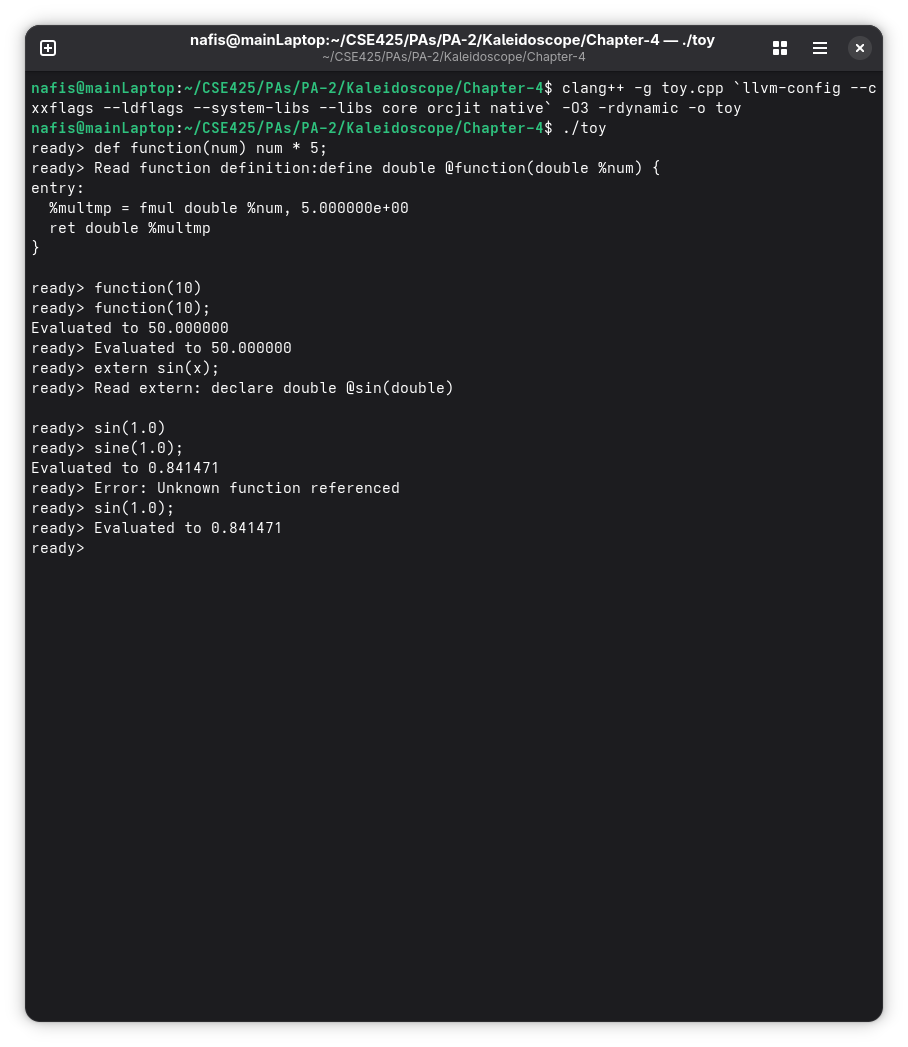
\includegraphics[width=0.55\linewidth]{./Ch-4.png}
  \caption{Kaleidoscope Terminal Output for JIT Compilation and Optimization}
  \label{fig:ch1-output}
\end{figure}


\subsection{Control Flow}
Kaleidoscope language is designed in such way it can be extended incrementally. New features are can be implemented without writing the whole compiler and can be only done by extending the lexer, parser, AST and LLVM code generation.

\textbf{If/The/Else:} Essentially the lexer is extended to support new keywords \verb|if, then| and \verb|else|. The parser adds a production function like \verb|ifexpr ::= 'if'| expression \verb|'then'| expression \verb|'else'| expression. The code generator implements this by creating three basic blocks, \verb|then, else| and \verb|merge|.A conditional branch then decides between \verb|then| or \verb|else| and a $\phi$ function in the \verb|merge| selects the correct value and returns it. 

\textbf{For loop:} Loop introduces a new variable i and initializes it  with \verb|<start>| repeatedly executes a body until the step expression defined as \verb|<end>| becomes false.
\begin{center}
\begin{minipage}{0.5\textwidth}
\begin{verbatim}
for i = <start>, <end>, <step> in <body>
\end{verbatim}
\end{minipage}
\end{center}
The compiler recognizes the for and in keywords, constructs a \verb|ForExprAST| node with fields for the loop variable's name, start, end, step and body. it gives that node the shape of a standard for loop with an entry block that branches to a loop block, a loop block that computes the body and the next value of the induction variable, a conditional branch that either jumps back to the loop header or exits to the next block and a return from the for expression.

\begin{figure}[H]
  \centering
  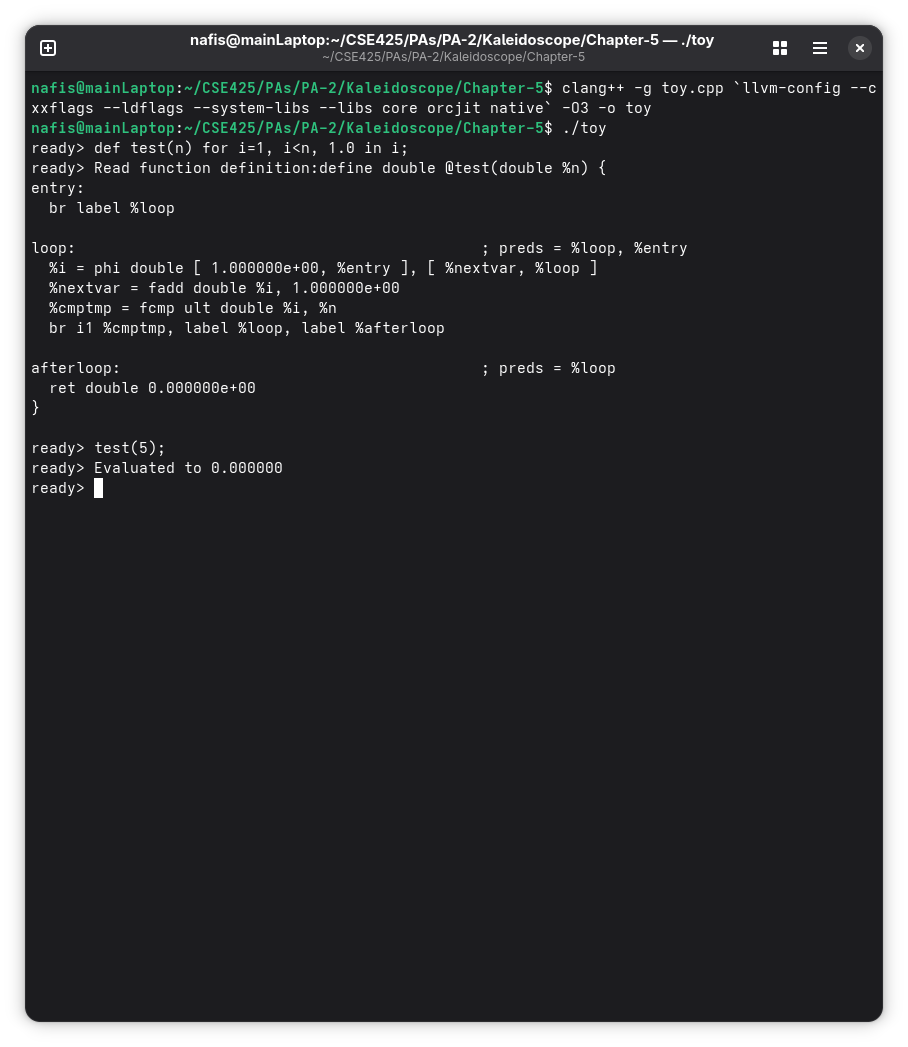
\includegraphics[width=0.55\linewidth]{./Ch-5.png}
  \caption{Kaleidoscope Terminal Output for Control Flow}
  \label{fig:ch1-output}
\end{figure}


\subsection{User-defined Operator}
Unlike traditional programming language like C++, Kaleidoscope lets the user define new ones directly in the source code. The language supports both binary operators and unary operators. An example can be for programmable unary and binary operators are as follows:
\begin{lstlisting}[language=C++]
# Logical unary not.
def unary!(v)
  if v then
    0
  else
    1;

# Define > with the same precedence as <.
def binary> 10 (LHS RHS)
  RHS < LHS;

# Binary "logical or", (note that it does not "short circuit")
def binary| 5 (LHS RHS)
  if LHS then
    1
  else if RHS then
    1
  else
    0;
\end{lstlisting}
Although these looks like normal function definitions, but the special forms \verb|unary!| and \verb|binary> 10| tell the front-end that these are operator definitions. The lexer recognizes the keywords \verb|unary| and \verb|binary,| the parser interprets the operator character and any optional precedence number and the prototype AST node \verb|PrototypeAST| records whether the declaration is for a normal function, a unary operator or a binary operator. Binary operators also store their precedence so they can be integrated into the existing precedence table used by the expression parser.

\begin{figure}[H]
  \centering
  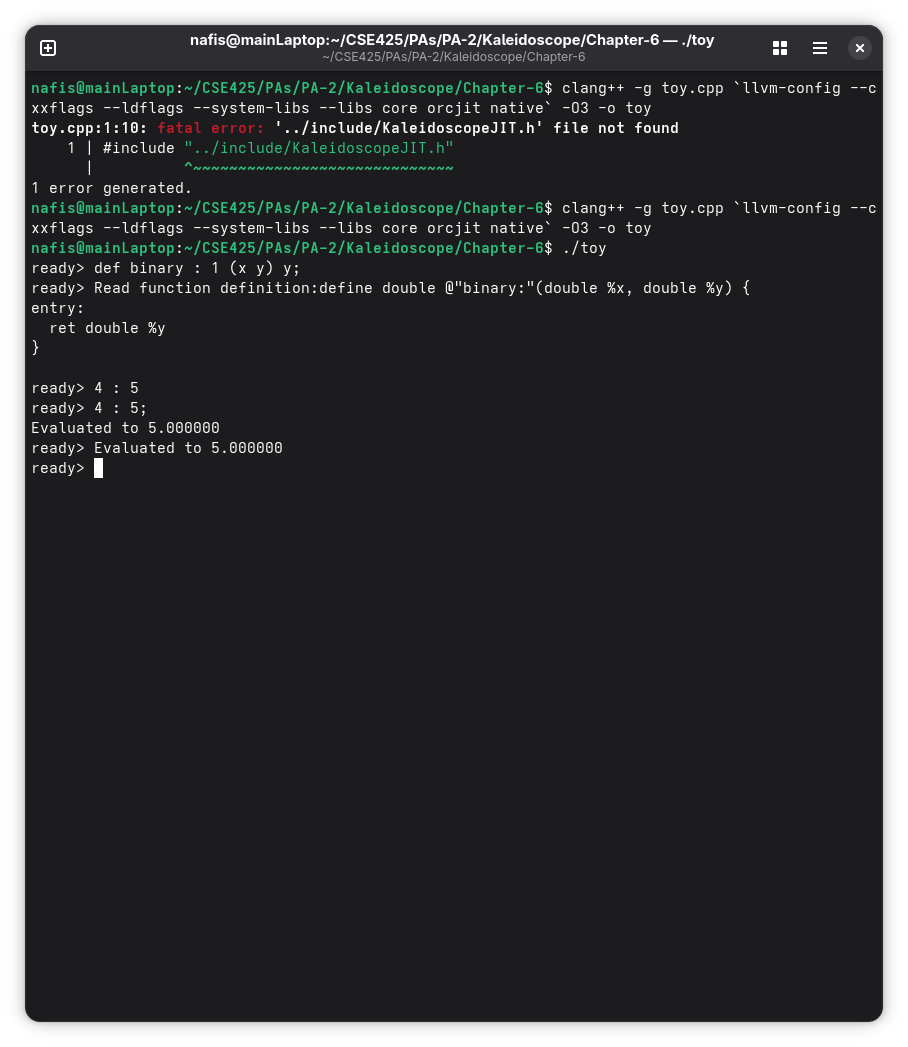
\includegraphics[width=0.55\linewidth]{./Ch-6.png}
  \caption{Kaleidoscope Terminal Output for User-defined Operator}
  \label{fig:ch1-output}
\end{figure}


\subsection{Mutable Variable}
Initially, the symbol table \verb|NamedValues| mapped each variable name directly to an LLVM Value*. Meaning that it always points to the "current" value. In order to make variable mutable, \verb|NamedVariables| is changed to maps each name to a stack slot \verb|alloca|.

This is done by a helper function as follows.
\begin{lstlisting}[language=C++]
/// CreateEntryBlockAlloca - Create an alloca instruction in the entry block of
/// the function.  This is used for mutable variables etc.
static AllocaInst *CreateEntryBlockAlloca(Function *TheFunction, StringRef VarName) {
  IRBuilder<> TmpB(&TheFunction->getEntryBlock(), TheFunction->getEntryBlock().begin());
  return TmpB.CreateAlloca(Type::getDoubleTy(*TheContext), nullptr, VarName);
}
\end{lstlisting}
With the change in place, variable reference no longer uses the stored Value* directly. Instead, code generation loads from the \verb|alloca| for that variable. Function arguments and loop induction variables are also stored into allocas at the start of the function or loop, so they can be changed later.

Once variables live in memory, an assignment such as \verb|x = expr| is simple: first evaluate \verb|expr|, then store the result into the \verb|alloca| for \verb|x|. In the parser, this assignment expression is resolved as a binary operator with low precedence. In \verb|BinaryExprAST::codegen()|, the ’\verb|=|’ case is detected and code is emitted that performs a store instead of an arithmetic operation.

In order to introduce new local variables, kaleidoscope adds a \verb|var\in| 
\begin{lstlisting}
var a = 1 in ...
\end{lstlisting}
This expression defines one or more variables (optionally with intial values) and then evaluates the body expression that can use those names. The AST stores a list of (name,initializer) pair and the body. The compiler works this way:
\begin{itemize}
\item Creates an \verb|alloca| for a variable
\item Stores the initializer
\item Adds the name and its \verb|alloca| to \verb|NamedValues|
\item Emits the code for the body
\end{itemize}
At this point, all mutable variables are implemented as loads and stores to stack slots. But this is inefficient. So, Kaleidoscope uses LLVM's \verb|mem2reg| optimization pass. This pass looks for simple allocas in the entry block whose addresses are only used by load and store. Then it automatically promotes them to SSA registers and inserts $\phi$ nodes where control flow joins. This way, the front end always emits simple \verb|alloca|-based code for mutable variables, and LLVM rewrites it into an efficient SSA form.

\begin{figure}[H]
  \centering
  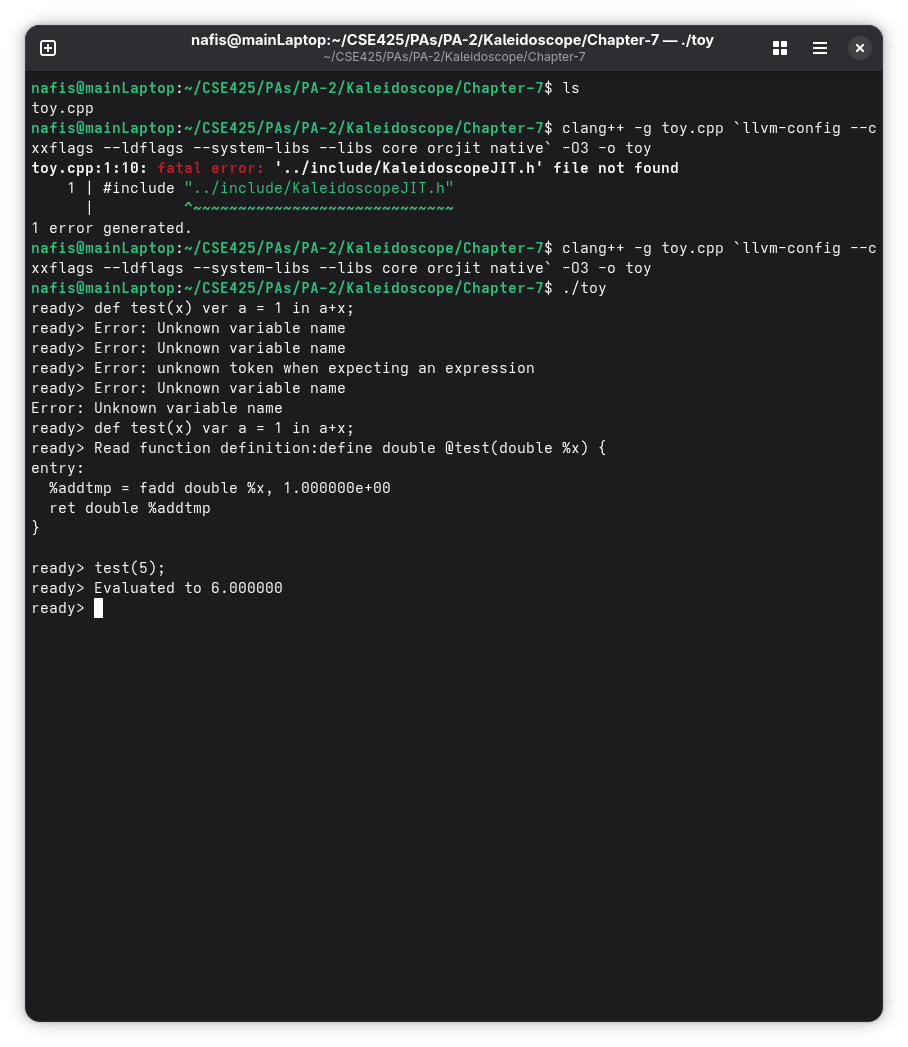
\includegraphics[width=0.55\linewidth]{./Ch-7.png}
  \caption{Kaleidoscope Terminal Output for Mutable Variable}
  \label{fig:ch1-output}
\end{figure}


\subsection{Object File Generation}
In Kaleidoscope, we can compile the IR Ahead-Of-Time to an object file instead of running it in the JIT. To do this, LLVM must know the target machine. LLVM uses a string called \textit{target triple}. This takes the form \verb|<arch><sub>-<vendor>-<sys>-<abi>| 

LLVM provides \verb|sys::getDefaultTargetTriple|, which returns the target triple of the current machine. This is a string that describes the CPU, vendor, operating system and Application Binary Interface (ABI).
\begin{lstlisting}[language=C++]
auto TargetTriple = sys::getDefaultTargetTriple();
\end{lstlisting}

LLVM doesn’t require to link in all the target functionality. If we only targeting certain architectures, we can only link in the functionality for those architectures. As example, we initialize all these targets for emitting object code.
\begin{lstlisting}[language=C++]
InitializeAllTargetInfos();
InitializeAllTargets();
InitializeAllTargetMCs();
InitializeAllAsmParsers();
InitializeAllAsmPrinters();
\end{lstlisting}

Additionally we need a \verb|TargetMachine|. \verb|TargetMachine| object describes the CPU and code generation option. One example follows using generic CPU and without any additional features.
\begin{lstlisting}[language=C++]
std::string Error;
auto Target = TargetRegistry::lookupTarget(TargetTriple, Error);
// Print an error and exit if we couldn't find the requested target.
// This generally occurs if we've forgotten to initialise the
// TargetRegistry or we have a bogus target triple.
if (!Target) {
  errs() << Error;
  return 1;
}
auto CPU = "generic";
auto Features = "";
TargetOptions opt;
auto TargetMachine = Target->createTargetMachine(TargetTriple, CPU, Features, opt, Reloc::PIC_);
\end{lstlisting}

After that we configure out module that tells LLVM about data layout and target triple for optimization purpose.
\begin{lstlisting}[language=C++]
TheModule->setDataLayout(TargetMachine->createDataLayout());
TheModule->setTargetTriple(TargetTriple);
\end{lstlisting}

To obtain the object file we need to define a location for the object file to write and make a pass that will emit the object file. An example for \verb|output.o| can be as follows:
\begin{lstlisting}[language=C++]
//----------------------------------//
// Target Location for the object file
//----------------------------------//
auto Filename = "output.o";
std::error_code EC;
raw_fd_ostream dest(Filename, EC, sys::fs::OF_None);

if (EC) {
  errs() << "Could not open file: " << EC.message();
  return 1;  
}

//-------------------------//
// Pass to emit object file
//-------------------------//
legacy::PassManager pass;
auto FileType = CodeGenFileType::ObjectFile;

if (TargetMachine->addPassesToEmitFile(pass, dest, nullptr, FileType)) {
  errs() << "TargetMachine can't emit a file of this type";
  return 1;
}

pass.run(*TheModule);
dest.flush();
\end{lstlisting}

Finally we get the output.o object file. This is a normal object file that can be linked with other C++ program. A snippet can be seen in the following snapshot.  
\begin{figure}[H]
  \centering
  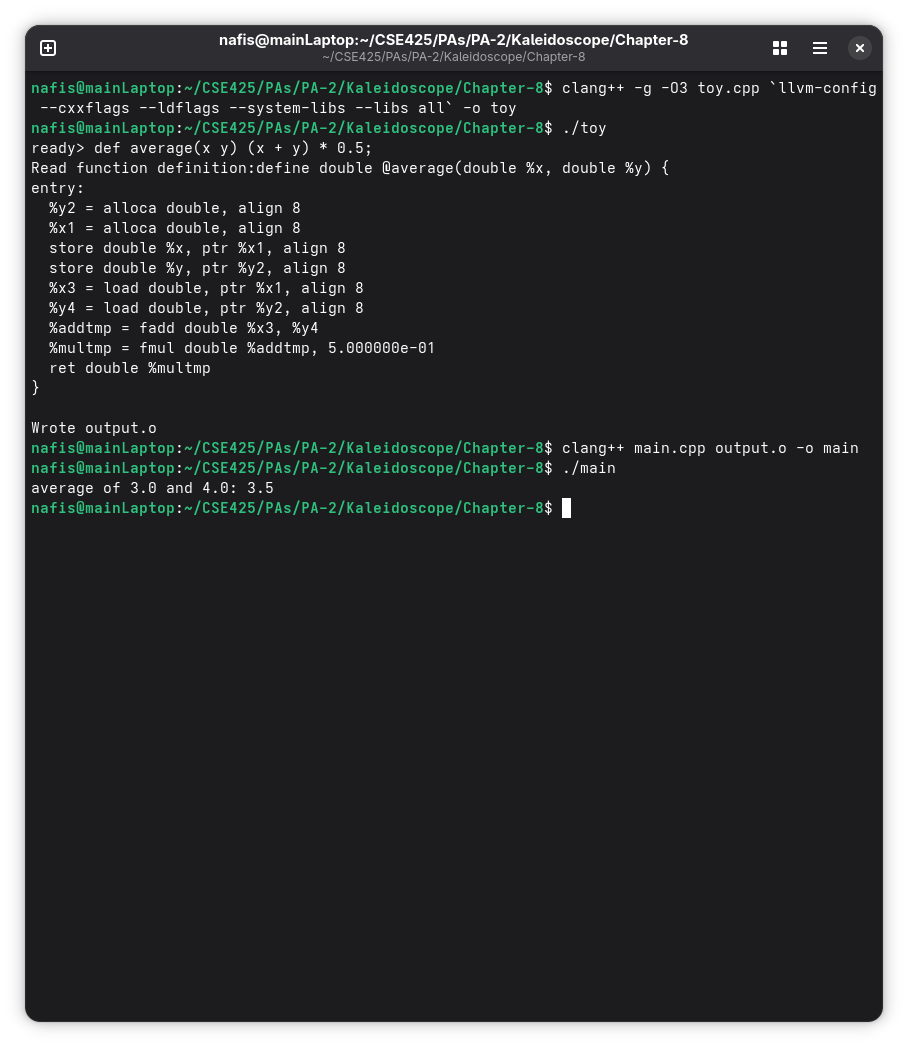
\includegraphics[width=0.55\linewidth]{./Ch-8.png}
  \caption{Kaleidoscope Terminal Output for Object File Generation}
  \label{fig:ch1-output}
\end{figure}
Here, the \verb|main.cpp| file is just a simple C++ file with a \verb|cout()| function and an \verb|extern| to use the Kaleidoscope function.

\begin{lstlisting}[language=C++]
#include <iostream>

extern "C" {
    double average(double, double);
}

int main() {
    std::cout << "average of 3.0 and 4.0: " << average(3.0, 4.0) << std::endl;
}
\end{lstlisting}


\subsection{Debug Information}
Like all the real programming language, we can extend the LLVM for the Kaleidoscope language to support debugging. Source level debugging uses formatted data that helps a debugger translate from binary and the state of the machine back to the source. LLVM uses a format called \textit{Debugging With Arbitrary Record Formats} (DWARF). DWARF is a compact encoding that stores types, source locations, variable locations, and function location. It lets the debugger map machine code  to source code.

\subsubsection{Switching to AOT Mode:} Debugging is a hard problem mainly because of the optimization. It makes keeping the track of source location difficult and can move variables in ways that are either, optimized out, shared in memory with other variables, or difficult to track. So, this part of the tutorial switches from the interactive REPL, to a simple ahead of time mode. Instead of the regular behaviour, compiler now reads a Kaleidoscope file, generates IR and then writes the IR to standard output. To have this new pipeline some changes were made.
\begin{itemize}
\item Make a anonymous function that contains the top level statement to be \verb|main|
\item Remove command line code wherever exists.
\item Disable all optimization pass and JIT.
\end{itemize}
With these changes, we can get executable program of the Kaleidoscope language with the following command:
\begin{lstlisting}
Kaleidoscope-Ch9 < fib.ks | & clang -x ir -
\end{lstlisting}

\textit{Buidling Debug information:} Similar to \verb|IRBuilder| class, LLVM provides us with a helper class \verb|DTBuilder|. We also create a container to keep cache for the frequent data. i.e., compile uni and type for \verb|double|
\begin{lstlisting}[language=C++]
static std::unique_ptr<DIBuilder> DBuilder;

struct DebugInfo {
  DICompileUnit *TheCU;
  DIType *DblTy;

  DIType *getDoubleTy();
} KSDbgInfo;

DIType *DebugInfo::getDoubleTy() {
  if (DblTy)
    return DblTy;

  DblTy = DBuilder->createBasicType("double", 64, dwarf::DW_ATE_float);
  return DblTy;
}

\end{lstlisting}

Then we construct the module. The compile unit is the top level debug container for source file.
\begin{lstlisting}[language=C++]
DBuilder = std::make_unique<DIBuilder>(*TheModule);

KSDbgInfo.TheCU = DBuilder->createCompileUnit(
    dwarf::DW_LANG_C, DBuilder->createFile("fib.ks", "."),
    "Kaleidoscope Compiler", false, "", 0);
\end{lstlisting}

While we’re producing a compile unit for the language Kaleidoscope, we used the language constant for C. This is because a debugger would not necessarily understand the calling conventions or default ABI for a language it does not recognize. Since we follow the C ABI in our LLVM code generation so it’s the closest thing to accurate.

Lastly, we call the \verb|finilize()| to get the debug information via \verb|DIBuilder| after our required information are finalized.
\begin{lstlisting}[language=C++]
DBuilder->finalize();
\end{lstlisting}

\textit{Functions:} For all the function we create a \verb|DISubprogram| node that with some metadata. In \verb|FunctionAST::codegen()| function we write some code to describe a context for the subprogram. The codes are follows:
\begin{lstlisting}[language=C++]
DIFile *Unit = DBuilder->createFile(KSDbgInfo.TheCU->getFilename(), KSDbgInfo.TheCU->getDirectory());

DIScope *FContext = Unit;
unsigned LineNo = 0;
unsigned ScopeLine = 0;
DISubprogram *SP = DBuilder->createFunction(
    FContext, P.getName(), StringRef(), Unit, LineNo,
    CreateFunctionType(TheFunction->arg_size()),
    ScopeLine,
    DINode::FlagPrototyped,
    DISubprogram::SPFlagDefinition);
TheFunction->setSubprogram(SP);
\end{lstlisting}
This lets the debugger to have a reference to all our metadata for the function.

\textit{Source Locations:} The most important thing for debug information is accurate source location which makes it possible to map to the source code back. Since the language does not have any mechanism to have any source location in the lexer or parser, it needed to be implemented. The following code does this job.
\begin{lstlisting}[language=C++]
struct SourceLocation {
  int Line;
  int Col;
};
static SourceLocation CurLoc;
static SourceLocation LexLoc = {1, 0};

static int advance() {
  int LastChar = getchar();

  if (LastChar == '\n' || LastChar == '\r') {
    LexLoc.Line++;
    LexLoc.Col = 0;
  } else
    LexLoc.Col++;
  return LastChar;
}
\end{lstlisting}

Now by editing all the AST nodes, all the classes will have the ability  to store source location.
\begin{lstlisting}[language=C++]
class ExprAST {
  SourceLocation Loc;

  public:
    ExprAST(SourceLocation Loc = CurLoc) : Loc(Loc) {}
    virtual ~ExprAST() {}
    virtual Value* codegen() = 0;
    int getLine() const { return Loc.Line; }
    int getCol() const { return Loc.Col; }
    virtual raw_ostream &dump(raw_ostream &out, int ind) {return out << ':' << getLine() << ':' << getCol() << '\n';
 }
\end{lstlisting}

To make sure that every instruction gets proper source location information, we have to tell \verb|Builder| whenever we are at a new source location. We use this helper function for this:
\begin{lstlisting}[language=C++]
void DebugInfo::emitLocation(ExprAST *AST) {
  if (!AST)
    return Builder->SetCurrentDebugLocation(DebugLoc());
  DIScope *Scope;
  if (LexicalBlocks.empty())
    Scope = TheCU;
  else
    Scope = LexicalBlocks.back();
  Builder->SetCurrentDebugLocation(
      DILocation::get(Scope->getContext(), AST->getLine(), AST->getCol(), Scope));
}
\end{lstlisting}

This sets the currect debug location and scope for all the following instructions that the builder emits.

\textit{variables:} Now that we have function, we need function arguments too. To make function argument visible to the debugger we also describe them as local variables and connect them to their \verb|alloca| instructions. This can be done we the following code:
\begin{lstlisting}[language=C++]
// Record the function arguments in the NamedValues map.
NamedValues.clear();
unsigned ArgIdx = 0;
for (auto &Arg : TheFunction->args()) {
  // Create an alloca for this variable.
  AllocaInst *Alloca = CreateEntryBlockAlloca(TheFunction, Arg.getName());

  // Create a debug descriptor for the variable.
  DILocalVariable *D = DBuilder->createParameterVariable(
      SP, Arg.getName(), ++ArgIdx, Unit, LineNo, KSDbgInfo.getDoubleTy(),
      true);

  DBuilder->insertDeclare(Alloca, D, DBuilder->createExpression(),
                          DILocation::get(SP->getContext(), LineNo, 0, SP),
                          Builder->GetInsertBlock());

  // Store the initial value into the alloca.
  Builder->CreateStore(&Arg, Alloca);

  // Add arguments to variable symbol table.
  NamedValues[std::string(Arg.getName())] = Alloca;
}
\end{lstlisting}

Now that we have developed a mechanism for the normal debugger like \verb|gdb| or \verb|lldb|, if we run a simple program under a debugger, we can do the following tasks.
\begin{itemize}
\item Set breakpoints on functions.
\item Step line by line through the Kaleidoscope source file.
\item Print argument values and variables while stopped at a point.
\end{itemize}

In summary, by adding a bit of location tracking and building a compile unit we turn the language something that can be debugged.



\section{Efficient Language Design Strategies}
The language Kaleidoscope is minimal by design, however it reflects classic goals of efficient programming language design. In this part of the report, we discuss the Kaleidoscope programming language in terms of the language design criteria.

\subsection{Readability}
The Kaleidoscope programming language uses small and consistent syntax which makes it readable. The core constructs of the language include function definitions, function calls, numeric literals and user-defined operators. Since, most of the operations are expressed in a mathematical style, arithmetic expression closely resemble their algebraic forms. However, the lack of distinct data types and error messages restricts readability when the language is extended.

\subsection{Writability}
The writability of the Kaleidoscope language is high owing to the rules of avoiding complex syntax. Almost everything is an expression in this language. So users do not have to learn any separate syntactic statement form. Defining a function requires only a prototype and a single expression body. The language also allows language extension via the tutorial with new operators and precedence which is immediately supported by the existing parser and AST. While the fundamental setback is that all values are treated as floating-point numbers with double precision, which restricts programs that rely on precision type.

\subsection{Reliability}
A program is said to be reliable if it performs to its specifications under all possible conditions. Kaleidoscope's reliability is minimal by design. The language does not perform type checking and treats all value as a floating-point number with double precision. Aliasing does not arise in the language because variables are local bindings lowered to separate LLVM IR allocations. Since there is no points, references, shared objects does not exists in the design. Also there is no exception handling to cause runtime errors.

\subsection{Regularity}
\subsubsection{Orthogonality}
Orthogonality in a programming language means that a relatively small set of primitive constructs can be combined in a relatively small number of ways to build the control and data structures of the language. \cite{sebesta} This means the language should behave similarly in similar contexts in simple sense. Since most of the constructs can be combined freely and every function returns a value, every non-prototype form is an expression, and binary operations are implemented uniformly through the same AST class, this reduces the number of special cases in the language.
\subsubsection{Uniformity}
The language applies consistent syntactic and semantic rules. Function calls always use the sane syntax. Variables follows the same binding structure. Parentheses uniformly introduces primary expressions. Although the lack of different data types limits the expressiveness of the language, it increases the uniformity.
\subsubsection{Generality}
In Kaleidoscope language, user-defined operators uses the same AST, parsing logic and code generation pipeline that built-in operators use. Function prototypes, function definitions, and expressions share a unified representation in the parser and code generator. This generality keeps the implementation compact and predictable.

\section{Modification}
This section of the report explains the modification that has been made to the Kaleidoscope language implementation. Explicit \verb|Boolean Literals| and a \verb|Modulo Operator| was introduced.

\subsection{Boolean Literal Extension}
Kaleidoscope usually handles floating-point number as \verb|0.0| as false and non-zero values as true. To improve readability we explicitly impose of \verb|true| and \verb|false| as keywords. This improves the Writability by mapping the keywords directly to the numeric constant values.

The lexer assigns new token values for \verb|true| and \verb|false|:
\begin{lstlisting}[language=C++]
enum Token {
...
tok_true = -13,
tok_false = -14
};

// inside gettok()
if (IdentifierStr == "true") return tok_true;
if (IdentifierStr == "false") return tok_false;
\end{lstlisting}

Generated tokens then handled by \verb|ParsePrimary()| and translates them into numeric AST
\begin{lstlisting}[language=C++]
case tok_true:
	getNextToken();
    return std::make_unique<NumberExprAST>(1.0);
case tok_false:
    getNextToken();
    return std::make_unique<NumberExprAST>(0.0);
\end{lstlisting}

Since, \verb|NumberExprAST| already emits LLVM IR emits for floating-point constants, no code generation required.
\begin{figure}[H]
  \centering
  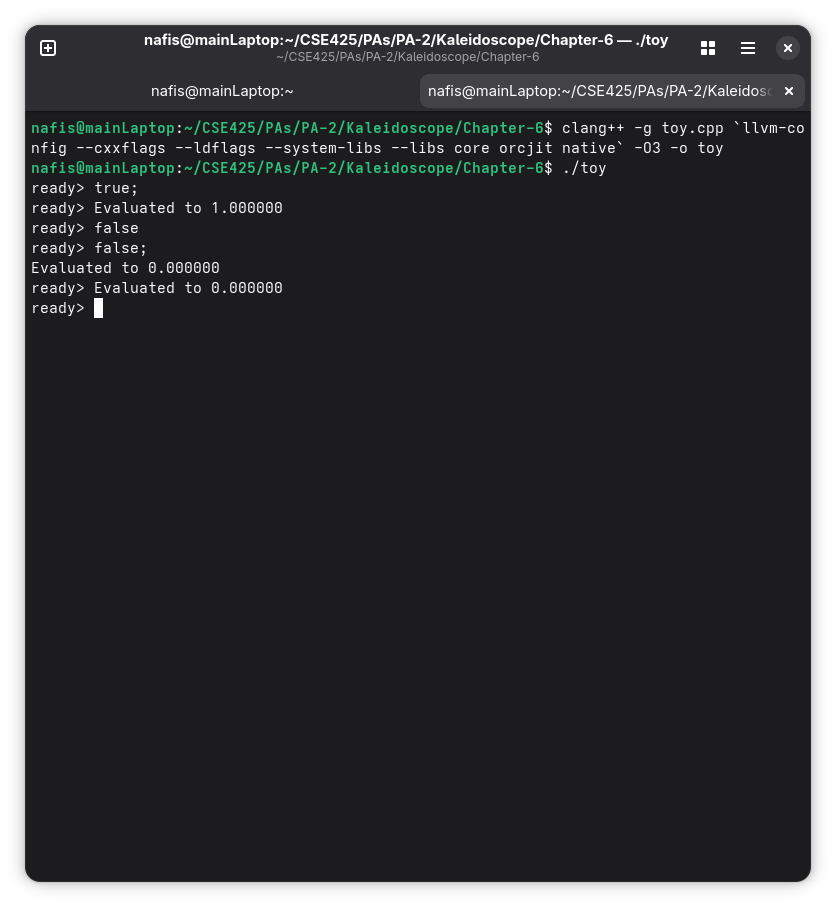
\includegraphics[width=0.55\linewidth]{./mod-1-bool.png}
  \caption{Kaleidoscope Terminal Output for Modification of Boolean Literal}
  \label{fig:ch1-output}
\end{figure}

\subsection{Modulo Operator Extension}
Since the Kaleidoscope language lacks the operator so new operator was introduced. Modulo operator is very useful for parity checks, cyclic computations and countless numeric algorithms, as common as Euclidean Algorithm for GCD.

The operator is given a new precedence value in \verb|main()| function.
\begin{lstlisting}[language=C++]
BinopPrecedence['%'] = 100;
\end{lstlisting}

Then code generator emits LLVM's floating-point remainder instructions:
\begin{lstlisting}[language=C++]
// In, Value *BinaryExprAST::codegen() {...}

case '%':
	return Builder->CreateFRem(L, R, "modtmp");
\end{lstlisting}

\begin{figure}[H]
  \centering
  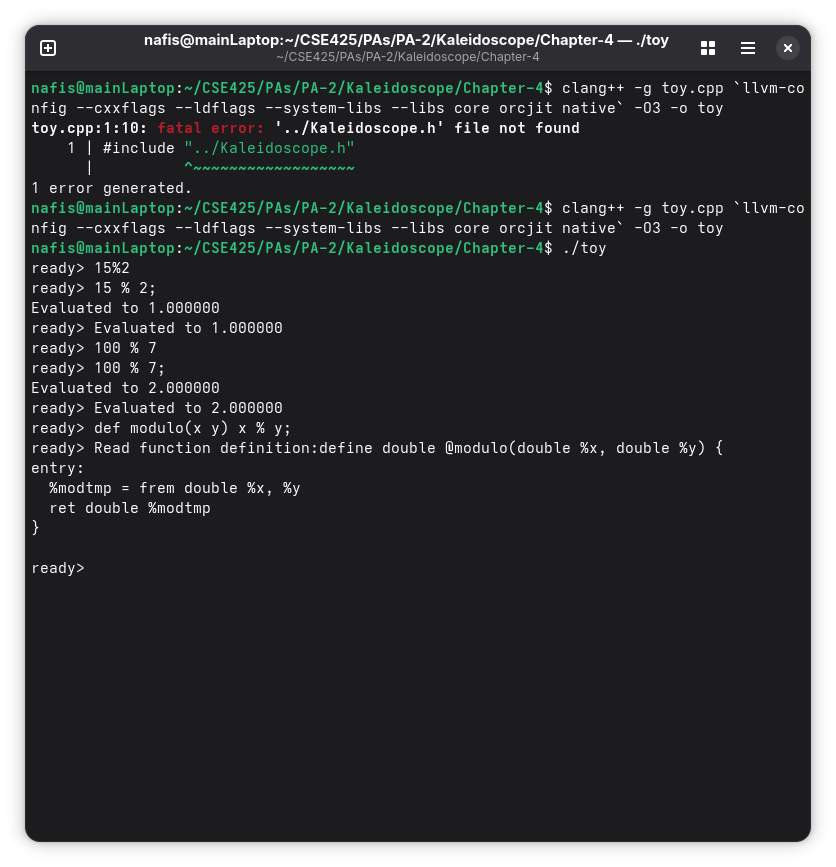
\includegraphics[width=0.55\linewidth]{./mod-2-mod.png}
  \caption{Kaleidoscope Terminal Output for Modification of Modulo Operator}
  \label{fig:ch1-output}
\end{figure}

Both the features requires minor modifications, While the lexer and parser absorbed most of the changes, LLVM IR handles the remaining part.

\begin{table*}[!htbp]
  \caption{Numbers of lines added}
  \label{tab:commands}
  \begin{tabular}{ccl}
    \toprule
    Features &Lines Added\\
    \midrule
    Boolean lit & 8 lines \\
    Modulo op & 2 lines\\
    \bottomrule
    Total & 10 lines
  \end{tabular}
\end{table*}


\section{Conclusion}
For this assignment, we implemented a small but complete programming language, Kaleidoscope with LLVM. This technical report documents the implementation and detailed analysis of the language. The language starts from a single expression language and as we built through a lexer, a parser with the combination of recursive-descent parsing and operator-precedence parsing, an abstract syntax tree and converted it to LLVM IR, implementation of both JIT compilation and ahead-of-time compilation to object file generation, so Kaleidoscope code can be run as a standalone executable.

The assignment reinforced several import compiler concepts including, lexing, parsing, operator precedence  handling, use of IR. For the LLVM, we explored basic blocks, SSA form, $\phi$ functions and optimization passes as well as JIT and ahead-of-time compilation.

Overall, the assignment provided hands-on exprience with language design decisions, LLVM IR, compiler optimizations, offering a deeper understanding of how high-level programs are translated into executable code.



\bibliographystyle{ACM-Reference-Format}
\bibliography{refs}


\end{document}

\endinput
